\chapter{Fundamental Discoveries}
\label{Discoveries-I}
In order to fully grasp the importance of major discoveries in particle physics, it is important to underline how, why and when they happened.

\section{Discovery of the positron}

In 1928, Paul Dirac published a paper introducing his famous equation, known as Dirac equation: the paper did not explicitly predict a new particle but did allow for electrons having either positive or negative energy as solutions. 
\vspace{2mm}

In 1932, thanks to Carl Anderson, the positron was discovered: he studied cosmic rays passing through a cloud chamber (Wilson chamber) and a lead plate. Through a magnetic field, he was able to distinguish different particles thanks to the different bending caused by their electric charge: doing so, he was able to detect a particle with a charge-over-mass ratio similar to the one of electrons, but with a positive charge, as shown in figure \ref{fig:positron}. Anderson observed a positive-charge particle traveling from below, with a momentum of about \SI{63}{MeV/c} measured from its curvature radius, and then emerging with a momentum of \SI{23}{MeV/c}.

\begin{figure}[h!]
    \centering
    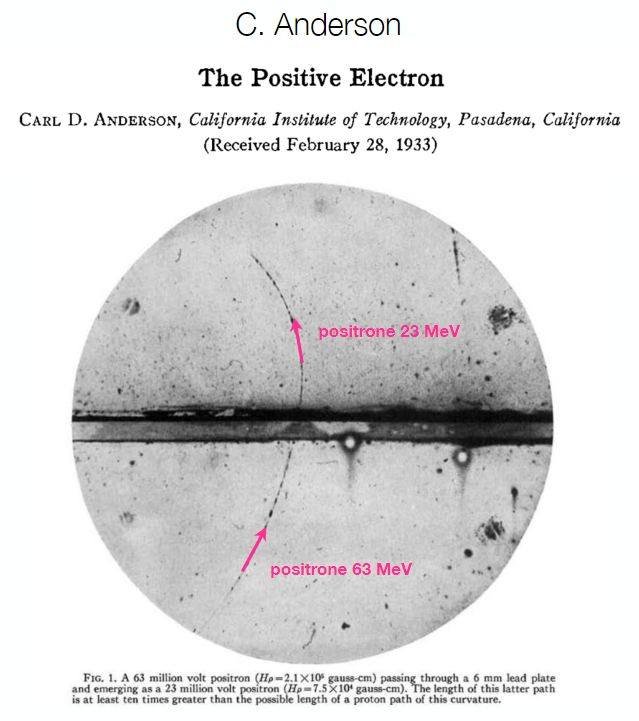
\includegraphics[width=0.5\textwidth]{Figures/FNSN16_1.JPG}
    \caption{A positron event photographed by Anderson in his Wilson chamber.}
    \label{fig:positron}
\end{figure}

The mass of the positron was obtained measuring the energy lost by the particle while interacting  with the lead plate, caused by bremsstrahlung.
The radiation length $X_0$ of lead (Pb) corresponds to $6 \ mm$, which is exactly the thickness of the lead plate chosen by Anderson.

Therefore, if the particle detected was an electron, we would expect an energy loss of $\approx 1/e$ of its initial energy (the momentum of the particle implies an energy above the critical energy for electrons in lead, \SI{7}{MeV}). Experimentally, the results were:
\begin{equation*}
    E_\text{entrance}(e^{+}) = 63 \ MeV \ \ \ \
    E_\text{exit}(e^{+}) = 23 \ MeV 
\end{equation*}
Consequently, the event observed is consistent to what expected for an electron, but with positive charge!

%Note that Dirac's equation is not going to be dealt with in these notes, while Klein Gordon equation (1926) and its implications will be discussed, including Dirac's way to solve them.
\section{Discovery of the neutron}
\subsection{Consequences of the discovery of the nucleus }
Rutherford's experiment was the first evidence of the existence of the atomic nucleus: its discovery inevitably led to the problem of defining its components and how they are kept together (i.e. how they interact).
%Since the total mass of the nucleus was a multiple of the mass of the proton, but the number of protons was fixed by the number of electrons ( to assure electrical neutrality), 
It was previously known that its mass was a multiple of the proton's mass, and its charge was a multiple of the elementary charge. However, since $M_{nucleus} > Z m_p$, it could not be made just of protons!
Consequently, other options had to be considered. First of all, the hypothesis of having some electrons confined inside the nucleus. Let's compute how much kinetic energy $T$ an electron should have for being inside the nucleus. The kinetic energy $T$ of one electron would be
\begin{equation*}
    T = E - m_e = \sqrt{m_e^2 + p^2}-m_e \approx p.
\end{equation*}
Considering $p \geq \Delta p$ and  $\Delta p \Delta x \geq \hslash$, a lower bound for $p$ can be found, using $\Delta x \simeq 1 \ fm$ (order of size of nucleus): the resulting kinetic energy is
\begin{equation*}
    T \approx p \geq \frac{\hslash}{\Delta x} \simeq \SI{200}{MeV}.
\end{equation*}

The final result is higher than the kinetic energy measured in nuclear phenomena: this hypothesis must therefore be wrong. In fact, $T_\text{measured}$ is approximately $T \geq 20 \ MeV$, for a particle as massive as a proton, but electrically neutral.

\subsection{Experiments 1930 - 1932}
In 1930, Bothe and Becker discovered that $\alpha$ particles passing through a berillium target ($^9_4Be$) were emitting a neutral and penetrating radiation. Since it was neutral, the first hypothesis considered to explain this radiation was $\gamma$ rays. However, this hypothesis could not justify the fact it was far more penetrating than expected.

Then, in 1932, Frédéric and Irène Joliot showed that these particles, going through paraffin, emitted high energy protons ($\sim \SI{5}{MeV}$), as in Figure \ref{fig:paraffin}. 

\begin{figure}[!h]
    \centering
    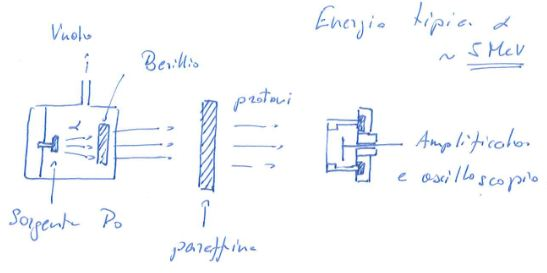
\includegraphics[width=0.9\textwidth]{Figures/FNSN16_2.JPG}
    \caption{Chadwick's experiment: $\alpha$ particles interact with berillium and produce a neutral radiation, which then interacts with paraffin producing protons with a typical energy of $\sim \SI{5}{MeV}$.}
    \label{fig:paraffin}
\end{figure} 

Meanwhile, all these evidences led Ettore Majorana in Rome to suppose that the particle could be a neutral version of the proton, the \emph{neutron}. 
The same year, James Chadwick performed an experiment, changing several targets, and proved the existence of a neutral particle, with approximately the same mass as a proton.
This discovery turned out to be fundamental for the development of nuclear physics.

It is easy to see that the kinetic energy needed for a photon or another particle with mass lower than the proton would be too much. Let's try to compute the maximum transmitted energy. 

\begin{figure}[!h]
    \centering
    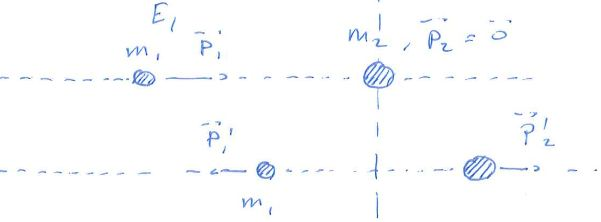
\includegraphics[width=0.7\textwidth]{Figures/FNSN16_3.JPG}
    \caption{Scattering configuration for Chadwick's experiment.}
    \label{fig:MaxEnergy}
\end{figure} 

As already seen for Bethe-Bloch equation in section \ref{sec:BB}, the maximum transmitted kinetic energy of the system described in Fig. \ref{fig:MaxEnergy} is
 \[ T_{\max} = \frac{2 m_2 p_1^2}{m_1^2 + m_2^2 + 2E_1m_2}\]
where we performed the substitution $E \rightarrow E_1, m \rightarrow m_2, M \rightarrow m_1, p \rightarrow p_1$.
Therefore from,
 \[ E_1 = T_1 + m_1,\]
 and
 \[ E_1^2 = p_1^2 + m_1^2.\]
 we get
 \begin{eqnarray*}
  p_1^2 &= (T_1 + m_1)^2 - m_1^2 \\
    & = T_1^2 + 2T_1m_1 + m_1^2 - m_1^2 \\
    & =T_1(T_1 + 2m_1).\\
\end{eqnarray*}
 Then, the final result is:
\[T_{\max} = T_1 \frac{2m_2(T_1 + 2m_1)}{(m_1 + m_2)^2 + 2T_1m_2}.\]
 
Curie and Joliot measured a recoil energy of approximately \SI{5}{MeV}.
Could this neutral radiation be caused by photons?
If particle $1$ is a photon, then $m_1 = 0$ and $m_2 \sim m_p$ (\SI{1}{GeV}), and $T_{\max}$ becomes
\[T_{max} = E_{\gamma} \frac{2E_{\gamma}m_2}{m_2^2 + 2E_{\gamma}m_2}.\]
 Therefore, $T_{max} \sim \SI{5}{MeV}$ would correspond to an energy of $\sim \SI{50}{MeV}$, too much to be caused by nuclear processes.
 Chadwick's experiment, which used a $^{14}N$ target ($m \sim \SI{14}{GeV}$), would have found
\[T_{\max} = 50 \cdot \frac{2 \cdot 50}{14\cdot10^3 + 2 \cdot 50 } \si{MeV} \ = \SI{0.35}{MeV}.\]
Instead, he measured $\sim \SI{1}{MeV}$.

Let's write the kinetic energy expected for hydrogen (paraffin) and nitrogen targets:
\begin{align*}
    T_H &= T_1 \frac{2m_H(2m_1 + T_1)}{(m_1 + m_H)^2 + 2T_1m_H},\\
    T_N &= T_1 \frac{2m_N(2m_1 + T_1)}{(m_1 + m_N)^2 + 2T_1m_N}.
\end{align*}
Their ratio, which depends on one unknown (the mass of the new, neutral particle), can be put equal to the experimental value:
\[ \frac{T_H}{T_N} = \frac{\SI{5}{MeV}}{\SI{1}{MeV}}= \frac{m_H}{m_N}\frac{(m_1 + m_N)^2 + 2T_1m_N}{(m_1 + m_H)^2 + 2T_1m_H}.\]
We can solve this equation to derive $m_1$: by considering that $T_1 \ll m_H,m_N$, one finds immediately that $m_1 \sim m_H = m_p$, i.e. that the mass of the neutron is very close to the proton mass.

\subsection{The neutron}
Accurately measured, the mass of the neutron is: 
\[m_n = (939.565379 \pm 0.000021) \si{MeV}\]
Then, the difference between $m_n$ and the mass of the proton $m_p$ is
\[m_n - m_p = (1.2933322 \pm 0.0000004) \si{MeV}\]
The fact that the two masses are almost the same resulted in a crucial element for particle physics.

Outside the nucleus, free neutrons are unstable and they decay into a proton, while emitting an electron ($e^{-}$) and an electron anti-neutrino ($\bar{\nu_e}$). The beta decay of the neutron, described above, can be denoted as follows:

\[ n \rightarrow p + e_{-} + \bar{\nu_e}.\]

The lifetime of the neutron is $\tau_n = (880.3 \pm 1.1) \si{s}$.

\section{Mesons: the muon and the pion}
\subsection{First experiments: Neddermeyer, Anderson, Street and Stevenson (1937) }
In the same years (1932), another important accomplishment was achieved in Cambridge, with the introduction of a ``trigger'' in cloud chambers. Triggering a cloud chamber, with two appropriately connected counters, means that the chamber could expand (and detect a particle) only when connected electronic tubes revealed the passage of a particle in the chamber itself (as showed in Fig. \ref{fig:trigger}). Using this technique, particles could actually take photographs of themselves!
 
\begin{figure}[!h]
    \centering
    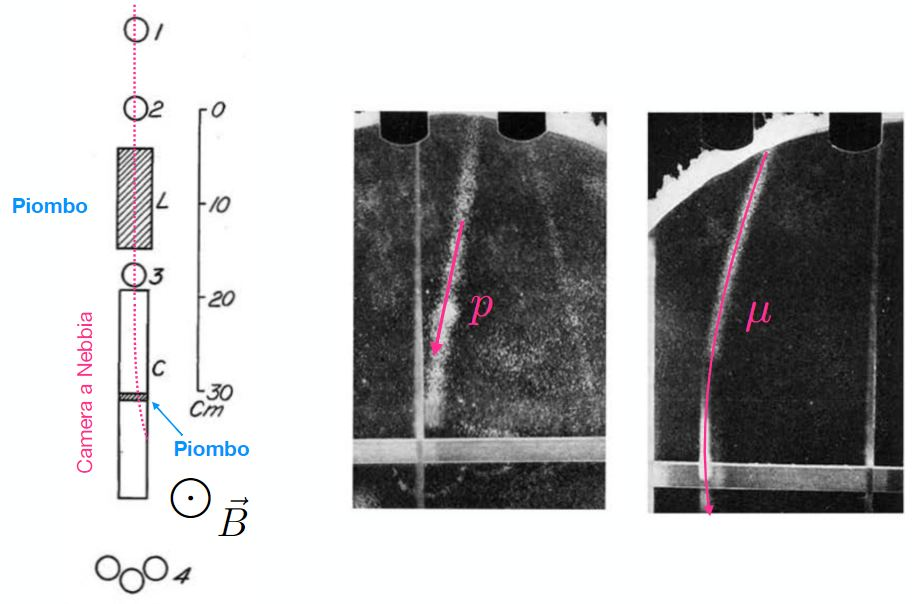
\includegraphics[width=\textwidth]{Figures/FNSN18_1.JPG}
    \caption{Cloud chamber: the principle of triggering}
    \label{fig:trigger}
\end{figure} 

This new apparatus was able to efficiently collect photographs of cosmic-ray particles and it proved to be fundamental for later discoveries.
In fact, in 1936 the American physicists Carl D. Anderson and Seth Neddermeyer detected a new particle using cosmic rays: it was named ``meson'', from \textit{mesos} (the Greek word for ``intermediate'') because its measured mass was between those of an electron and a proton. 
More accurate measurements enabled to define its value: Street and Stevenson deduced it by measuring its momentum and velocity.
Through the radius of curvature caused by a magnetic field, it was possible to measure the momentum of such particle. Instead, the velocity could be measured by comparing the energy of shower particles with the ionization energy released by the collisions with matter (see the low-velocity behaviour of the the Bethe-Bloch equation).

Yukawa had predicted the existence of a particle (the pion) of $m \sim 100-200 \si{MeV}$: could this new particle be the one he was looking for? It took a few years to prove it wasn't.

\subsection{The Conversi, Pancini and Piccioni experiment (CPP) and the Tomonaga and Araki theory (1940 - 1941) }

In 1941, Conversi and Piccioni developed a better version of the previous experiments to detect the meson, by splitting the particles according to their electric charge using ``magnetic lenses''.

\begin{figure}[!h]
    \centering
    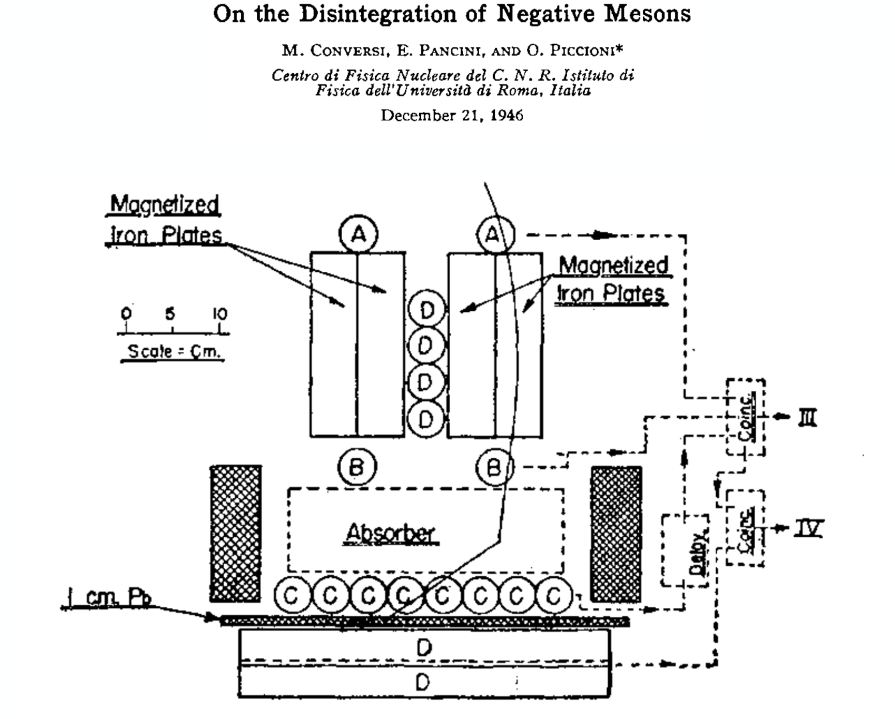
\includegraphics[width=\textwidth]{Figures/FNSN18_5.JPG}
    \caption{Experimental apparatus of the Conversi-Pancini-Piccioni experiment: positioning of counters, absorber and magnetized iron plates. All counters labeled as D are connected in parallel.}
    \label{fig:CPC}
\end{figure} 

The outcome of this experiment did not agree with the theory of Tomonaga and Araki (1940), denying the cosmic rays mesotron was actually the Yukawa meson (i.e. the particle used to explain the short-range nuclear force with the Yukawa potential).
This theory described the effect of the nuclear Coulomb field on the capture of slow mesons, stating that different charged mesons have a different behaviour when it comes to the competition between nuclear capture and spontaneous decay. Positive mesons would be repelled by the positive charge of the nucleus, and therefore would tend to encur in decays as in vacuum. %On the contrmore likely to decay in a short period and to interact less with the nucleus, thanks to the nuclear repulsion.

\begin{figure}[!h]
    \centering
    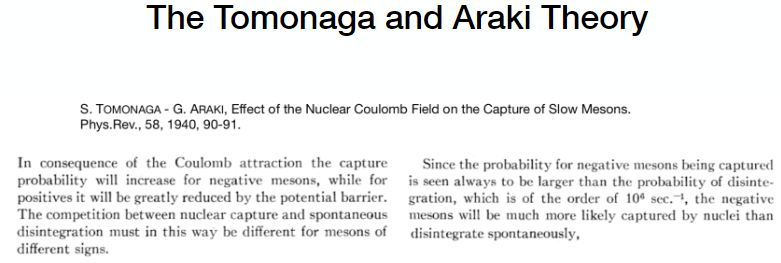
\includegraphics[width=\textwidth]{Figures/FNSN18_4.JPG}
    \caption{Tomonaga and Araki Theory article, published in 1940.}
    \label{fig:TAT}
\end{figure} 

Instead, according to Tomonaga and Araki, the capture probability would increase for negative mesons (by atoms with Bohr radius $ \frac{\hslash}{m_e c \alpha}$), that would be more likely to be attracted by the nucleus, interact with it and lose energy before decaying. Consequently, an anomalous absorption was to be detected: the first results, obtained using iron (Fe), apparently confirmed the theory. 

\begin{figure}[!h]
    \centering
    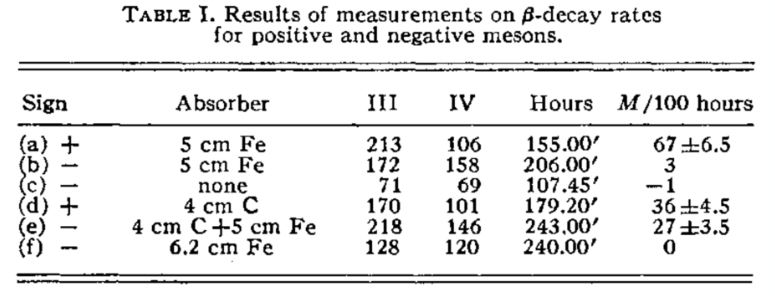
\includegraphics[width=0.9\textwidth]{Figures/FNSN18_7.JPG}
    \caption{Results of measurement of the Conversi-Pancini-Piccioni experiment with iron and carbon}
    \label{fig:Data}
\end{figure} 

It was only by switching material, passing from iron to graphite (C), that incompatible results came out (see Fig. \ref{fig:Data}): using carbon, negative particles behaved like positive ones, with a similar decay rate.
In 1942, Rasetti measured the mean life of this new particle as approximately $\tau \sim 1.5 \ \mu s$, as shown in Fig. \ref{fig:rasetti}.

\begin{figure}[!h]
    \centering
    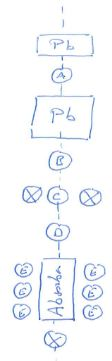
\includegraphics[width=0.2\textwidth]{Figures/FNSN18_3.JPG}
    \caption{Rasetti's apparatus to measure the mesotron mean life}
    \label{fig:rasetti}
\end{figure} 
\clearpage

\subsection{Nuclear interaction (1947)}

In 1947, D. H. Perkins performed other experiments using emulsions as shown in Fig. \ref{fig:Perkins}. His results seemed to confirm the hypothesis of nuclear interaction and capture discarded by Conversi's experiment. So, what is the nature of cosmic rays? 

\begin{figure}[!h]
    \centering
    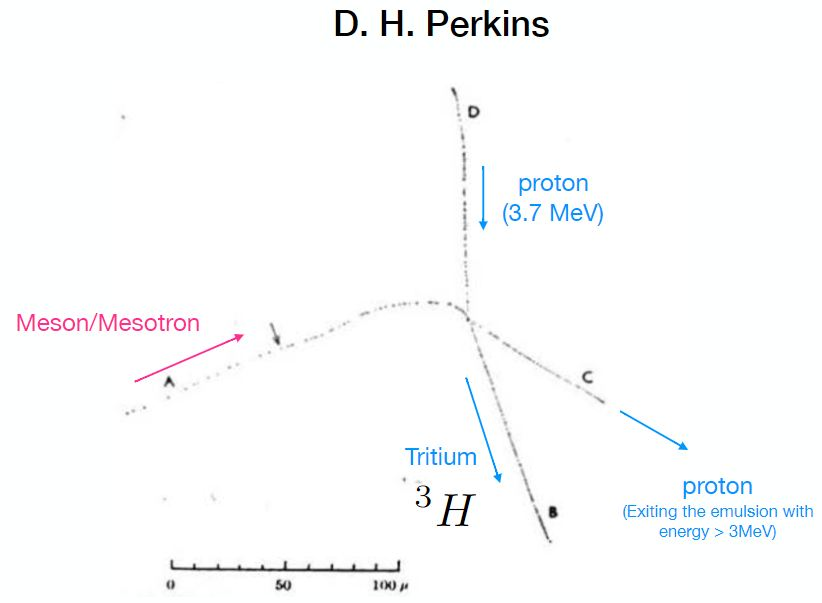
\includegraphics[width=0.6\textwidth]{Figures/FNSN18_8.JPG}
    \caption{D.H. Perkins emulsion experiment.}
    \label{fig:Perkins}
\end{figure} 

During the same year, Marshak and Bethe suggested the existence of two different particles: the pion and the muon. Meanwhile, Fermi, Teller and Weisskopf wrote an article called ``The Capture of Negative Mesotrons in Matter''\footnote{Phys. Rev 71, 314-315 (1947) (Fermi - Teller)}, explaining why the mesotron could not be the same particle as the Yukawa meson.
Finally, the problem was solved by Lattes, Muirhead, Occhialini and Powell. They observed an event showing the existence of two particles: the pion, predicted by Yukawa, and the muon.
It took a quarter of century to finally understand that the Yukawa force is not the fundamental strong nuclear interaction, and that the pion itself is a composite particle made of two elementary particles (quarks).

\begin{figure}[!h]
\begin{center}
    \centering
    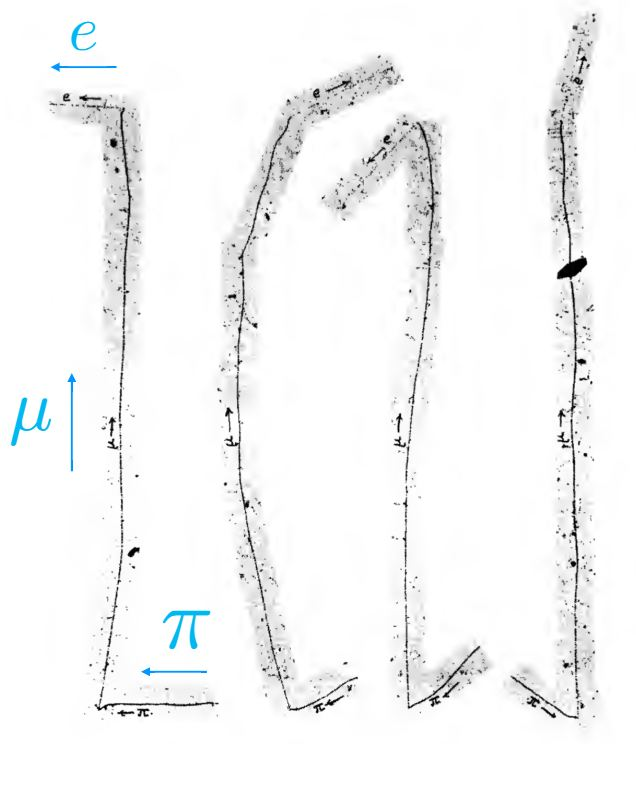
\includegraphics[width=0.6\textwidth]{Figures/FNSN18_9.JPG}
    \caption{Discovery of the pion}
    \label{fig:pione}
\end{center}
\end{figure}

When the American physicist Rabi heard the news of the discovery of the muon, he replied: ``Who ordered that?!''. In fact, it was not known why this new particle existed: why a particle should have the same charge as the electron, but bigger mass? After measuring all its properties, this question became quite relevant. Even today, we have no answer.

%\begin{comment}

\section{The discovery of Strangeness}

Until the 1940s, known particles included: $e^-$, $e^+$, $\gamma$, $p$, $n$ and the pion (and, later, the muon).

\begin{figure}[!h]
    \centering
    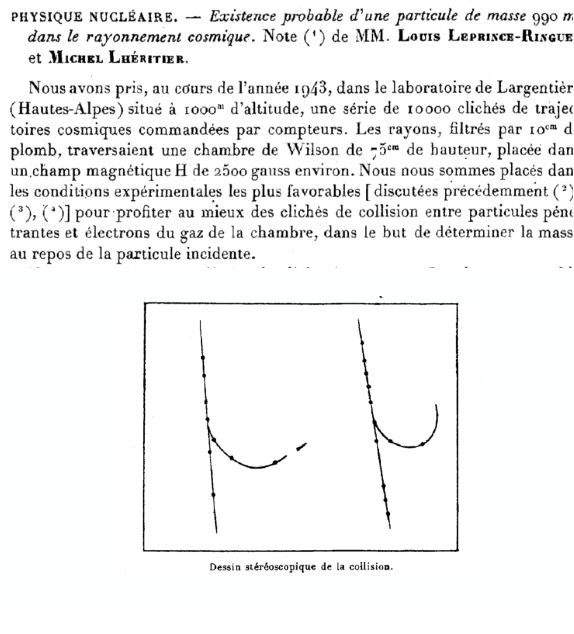
\includegraphics[width=0.6\textwidth]{Figures/FNSN27_1.JPG}
    \caption{Le Prince Ringuet and L'Héritier experiment in 1943}
\end{figure} 

In 1943, Leprince-Ringuet and L'Héritier, working in a laboratory on the Alps with a triggered cloud chamber \(\SI{75}{cm} \times \SI{15}{cm}\times\SI{10}{cm}\) in a magnetic field $B = \SI{0.25}{T}$, discovered a particle with a mass of $(506 \pm 61) \ MeV$.
The measurement was based on the event they observed in almost $10000$ photos, as shown in Fig. \ref{fig:LepRing}.

\begin{figure}[!h]
    \centering
    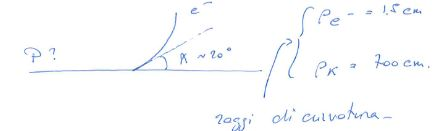
\includegraphics[width=0.8\textwidth]{Figures/FNSN27_2.JPG}
    \caption{Effect observed on 10000 photos by Leprince-Ringuet and L'Héritier}
    \label{fig:LepRing}
\end{figure} 


\begin{figure}[!h]
    \centering
    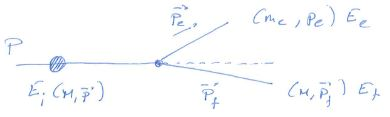
\includegraphics[width=0.6\textwidth]{Figures/FNSN27_3.JPG}
    \label{fig:setting1}
    \caption{Illustration of the scattering,described physically in this section}
\end{figure} 

Let's try to derive the mass $M$ from the setting described in Fig. \ref{fig:setting1}. Using the conservation of momentum and energy,
\[ \vec{p} = \vec{p_e} + \vec{p_f}, \]
\[E_i + m_e = E_e + E_f, \]
and so
\[E_f =  E_i + m_e - E_e.\]
Squaring both sides,
 \begin{eqnarray*}
&(E_i + m_e - E_e)^2 = E_f^2 = M^2 + p_f^2 = M^2 + (\vec{p}-\vec{p_e})^2, \\
&E_i^2 + m_e^2 + E_e^2 + 2 E_i m_e - 2E_i E_e -2E_e m_e = M^2 + p^2 + p_e^2 - 2p p_e cos{\chi}. \\
\end{eqnarray*}
Since $M^2 + p^2 = E_i^2$, then
\[m_e^2 + E_e^2 + 2 E_i m_e - 2E_i E_e -2E_e m_e = p_e^2 - 2p p_e cos{\chi}.\]
Let's add $m_e^2$ on both sides:
\[2m_e^2 + E_e^2 + 2 E_i m_e - 2E_i E_e -2E_e m_e= m_e^2 + p_e^2 - 2p p_e cos{\chi}.\]
Since $m_e^2 + p_e^2 = E_e^2$, then
\[2m_e^2 + 2 E_i m_e - 2E_i E_e - 2E_e m_e = - 2p p_e cos{\chi}.\]
Therefore we can write
\begin{eqnarray*}
 m_e(m_e + E_i) - E_e(m_e + E_i) & = -p p_e cos{\chi} \\
 (E_i + m_e)(E_e - m_e) &= p p_e cos{\chi}\\
 E_i + m_e & = \frac{ p p_e cos{\chi}}{E_e - m_e}
\end{eqnarray*}
Hence, considering $E_i \gg m_e$,
\begin{eqnarray*}
E_i^2 &\approx p^2(\frac{ p_e cos{\chi}}{E_e - m_e})^2,\\
M^2 + p^2 &= p^2 \frac{E_e^2 - m_e^2}{(E_e - m_e)^2}cos{\chi}^2,\\
M^2 &= p^2 \left[ \frac{E_e^2 - m_e^2}{(E_e - m_e)^2}cos{\chi}^2 - 1 \right],\\
\end{eqnarray*}
and the final expression is
\[ M = p \sqrt{\frac{E_e^2 - m_e^2}{(E_e - m_e)^2}cos{\chi}^2 - 1 } \sim 540 \ MeV.\]
The mass of this new particle was approximately half of the mass of the proton and four times bigger than the mass of the pion.

\begin{figure}[!h]
    \centering
    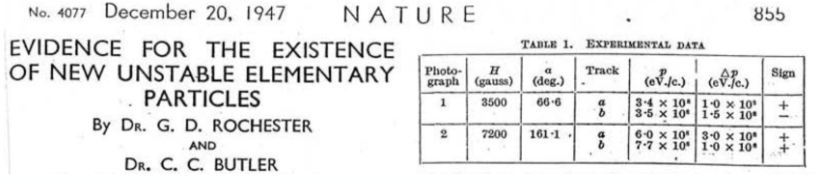
\includegraphics[width=0.9\textwidth]{Figures/FNSN27_4.JPG}
    \label{fig:Roc}
    \caption{Original paper by Rochester and Butler from 1947}
\end{figure} 

Only in 1947, it was possible to collect evidence of a neutral particle with similar mass: Rochester and Butler were able to detect the  decay
\[K^0_S \rightarrow \pi^+\pi^-, \]
Followed shortly after by
\begin{eqnarray*}
& K^{\pm} \rightarrow \mu^{\pm}\nu,\\
& K^{\pm} \rightarrow \pi^{\pm}\pi^{\pm}\pi^{\mp}.\\
\end{eqnarray*}

\begin{figure}[!h]
    \centering
    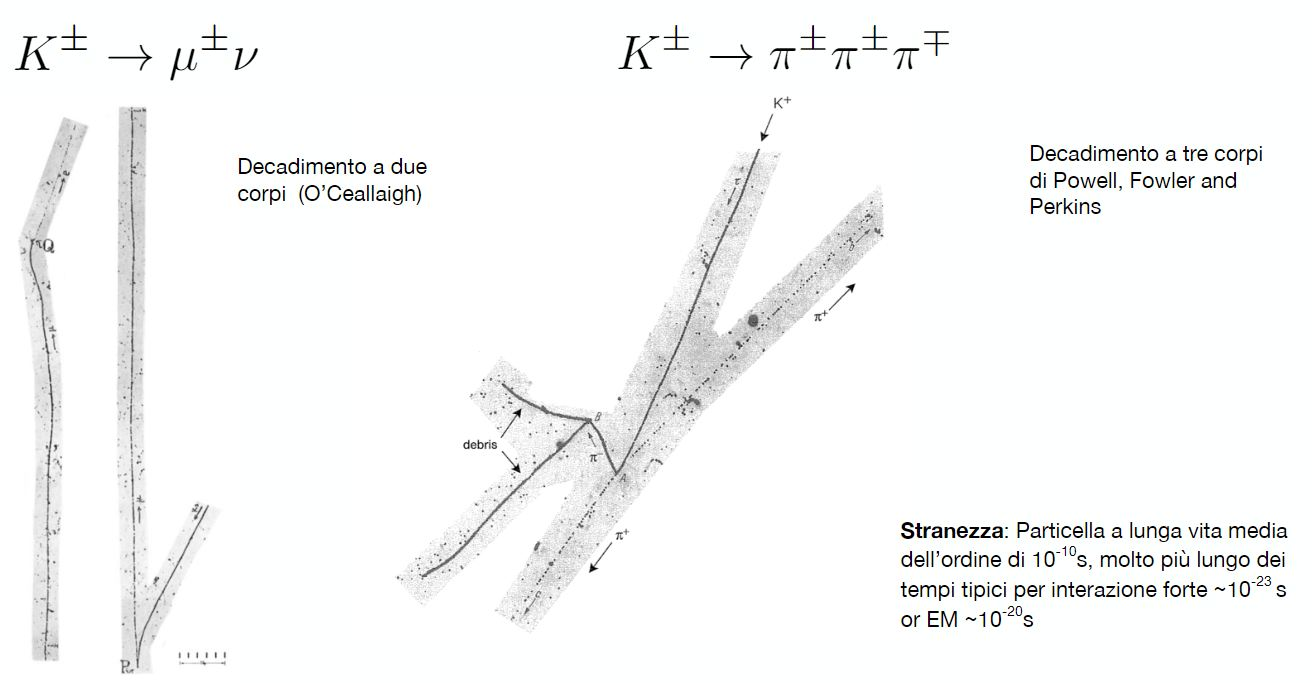
\includegraphics[width=\textwidth]{Figures/FNSN27_6.JPG}
    \label{fig:roc2}
    \caption{Picture of the other decays related to $\K^{\pm}$}
\end{figure} 

These particles were considered "strange" because their mean life is not compatible with strong interaction (i.e. it showed a slower decay than expected), while their final states contain strongly-interacting particles. In order to explain this particular behaviour, in the 1950s Pais introduced the idea of a new quantum number, called \emph{strangeness}, that  was preserved during their creation, but not conserved in their decay.

\begin{figure}[!h]
    \centering
    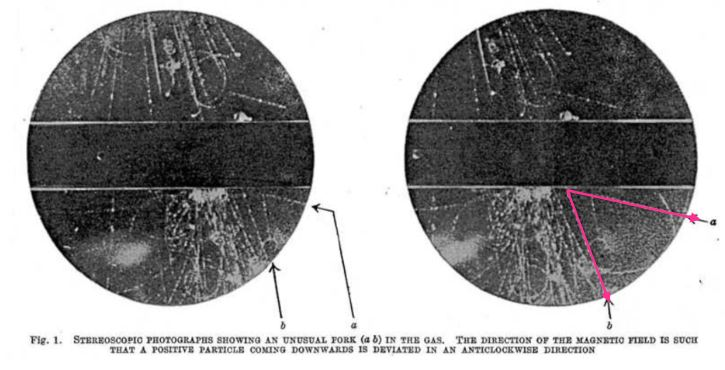
\includegraphics[width=0.6\textwidth]{Figures/FNSN27_5.JPG}
    \label{fig:roc1}
    \caption{Pictures from the Rochester-Butler experiment}
\end{figure} 
% VALERIO ARRIVED HERE


\section{Helicity and Wu experiment}
\subsection{Helicity}

One of the most important quantities regarding parity and symmetry is the projection of the angular momentum or the projection of the spin onto the direction of momentum, called helicity.

\[h = \frac{\vec{p}\cdot \vec{s}}{|\vec{p}\cdot \vec{s}|}  \]
This observable physical quantity is not conserved and is not Lorentz invariant: it is always possible for a massive particle to find a frame of reference where h changes sign.
However,for mass-less particle, the helicity seems to be a conserved quantity.
Furthermore, helicity is a \textbf{pseudo-scalar} quantity: in linear algebra, a pseudo-scalar is a quantity that behaves like a scalar, except that it changes sign under a parity inversion.
This notion will be crucial to understand Mme. Wu experiment, as well as for weak interactions theory and field theory (particularly for fermions).

\subsection{Wu experiment}

The Wu experiment was a nuclear physics experiment conducted in 1956 by the Chinese American physicist C.S. Wu. \ \
The experiment's purpose was to establish whether or not conservation of parity (P-conservation) also applied to weak interactions, through cobalt-60 (Co) $\beta$ - decay:

\[ ^{60}Co \rightarrow _{28}^{60}Ni^* + e^- +\bar{\nu_e}\]

The experiment was conducted at the cryogenic temperatures of approximately $10^{-3} \ K$, in order to preserve $^{60}Co$ polarization with a strong magnetic field $\vec{B}$.
In fact, a low temperature is necessary to satisfy the condition $\vec{\mu_B}\cdot \vec{B} \gg K_BT$. 

\begin{figure}[!h]
    \centering
    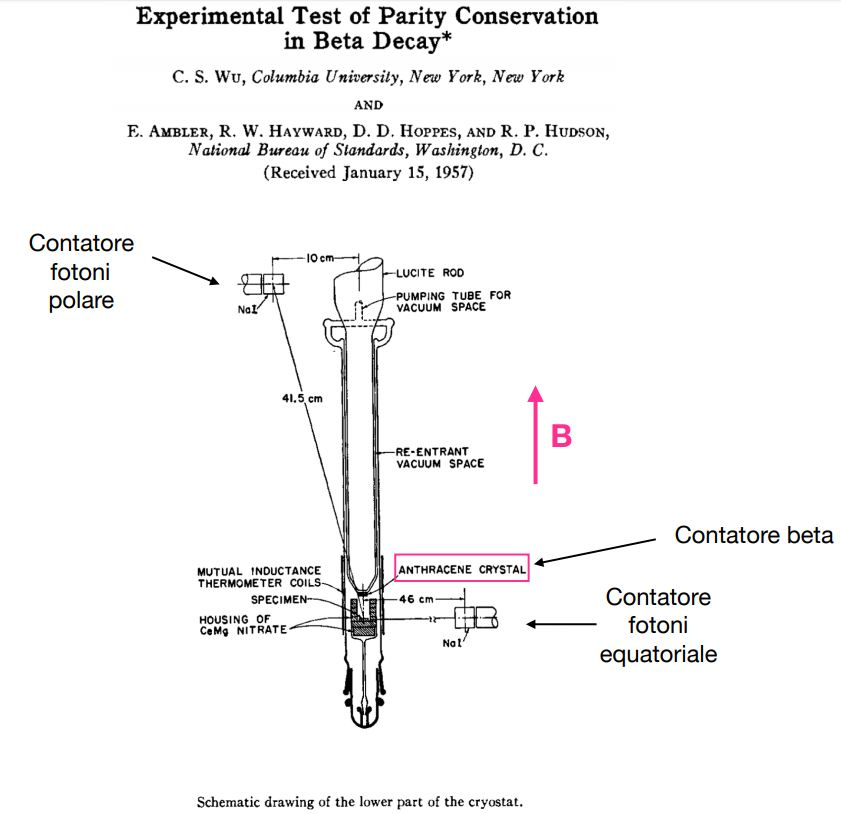
\includegraphics[width=0.6\textwidth]{Figures/FNSN31_1.JPG}
    
    \caption{Wu's experimental apparatus, with details of the cryostat}
    \label{fig:Wusetting1}
\end{figure} 

An other important feature of $^{60}Co$ is that it decays in an excited $^{60}Ni^*$ nucleus, that emits a photon: measuring the anisotropy of the photon emission, it is possible to measure the polarization of cobalt.

Photon and electrons counters (figure \ref{fig:Wusetting1}) reported a correlated asymmetry between the polarization of the source and the asymmetry of $\beta$-decays (even changing the polarization of the field). 
How can we explain the observations made?
Let's focus on figures \ref{fig:Wu1} and \ref{fig:Wu2}:

\begin{figure}[!h]
    \centering
    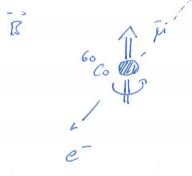
\includegraphics[width=0.3\textwidth]{Figures/FNSN31_2.JPG}
    \caption{Description of the cobalt decay}
    \label{fig:Wu1}
\end{figure} 

\begin{figure}[!h]
    \centering
    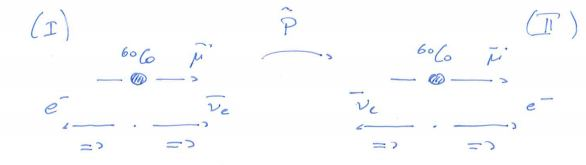
\includegraphics[width=0.6\textwidth]{Figures/FNSN31_3.JPG}
    \caption{Two possible configurations under parity of the cobalt decay }
    \label{fig:Wu2}
\end{figure} 

if parity is conserved, then both symmetrical configurations (I) and (II) should have the same rate. The experiment showed that only (I) was observed! Therefore, it proved that conservation of parity was violated by weak interaction.
Furthermore, for massless particles, helicity is Lorentz invariant: this conservation law could be extended to neutrinos, for their mass being $\sim 0$ compared to the other masses of standard model particles. Consequently, it could be produced only neutrino with helicity $-1$ (left-handed) or antineutrino with helicity +1 (right-handed).

\begin{figure}[!h]
    \centering
    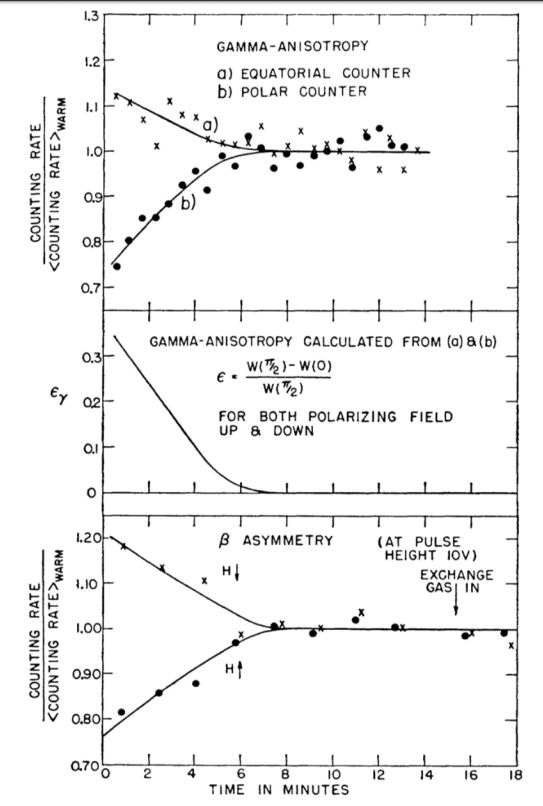
\includegraphics[width=0.4\textwidth]{Figures/FNSN31_4.JPG}
    \caption{Experimental data from the Wu experiment}
     \label{fig:Wu3}
\end{figure} 

Let's note that the material loses its polarization with the passing of time and the consequencial increasing in temperature (photons rate becomes equal to the one with higher temperature).
Let's consider that:

\begin{eqnarray*}
& ^{60}Co \rightarrow _{28}^{60}Ni^* + e^- +\bar{\nu_e}\\
&\hookrightarrow ^{60}Ni + \gamma
\end{eqnarray*}

\section{Discovery of resonances}

Considering both the development of accelerators and how high energy hadrons interact, during hadrons avalanches a big amount of particles is produced, like pions and kaons. 
These kind of particles can be selected (using a magnetic field) and collimated using shields to get a particle beam. These beams were used for fundamental discoveries in hadronic resonances. Figures \ref{fig:Wu4}, \ref{fig:Wu5} and \ref{fig:Wu6} show a few examples of experimental apparatuses and their results in terms of measured cross-section as a function of the center-of-mass energy.

\begin{figure}[!h]
    \centering
    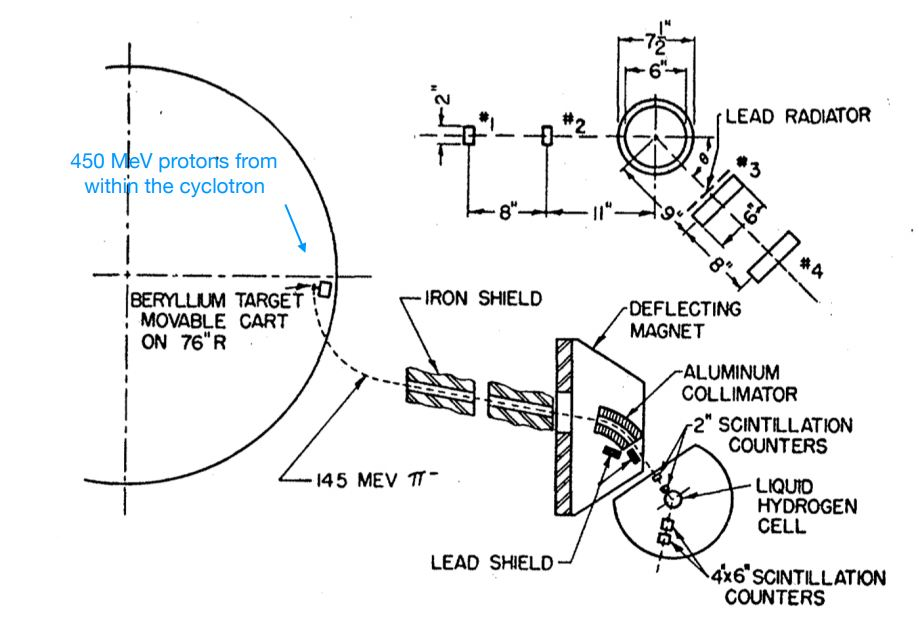
\includegraphics[width=0.6\textwidth]{Figures/FNSN31_5.JPG}
    \label{fig:Wu4}
    \caption{Experimental apparatus used in Chicago for the measurement of the $\pi^+p$ interaction cross section}
\end{figure} 

In 1955, in Berkeley, anti-protons were discovered  through particles beams: the importance of the discovery of the resonance is further discussed in chapter \ref{ch:conclusion}. 

\begin{figure}[h]
    \centering
    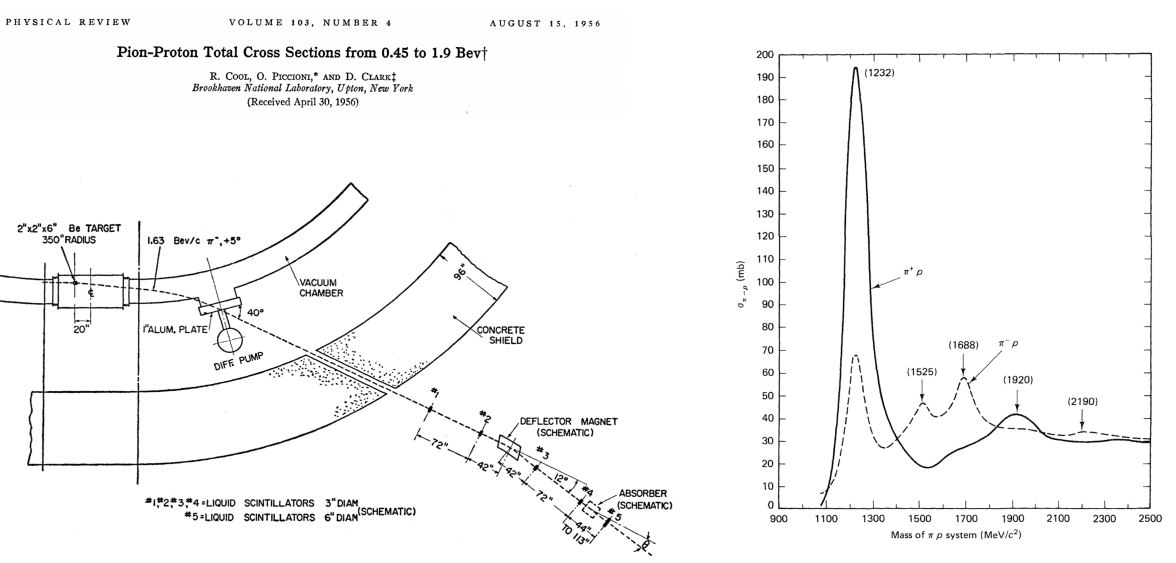
\includegraphics[width=0.8\textwidth]{Figures/FNSN31_6.JPG}
    \label{fig:Wu5}
    \caption{Resonances with strong isospin produced in the $\pi^- p$ interaction.}
\end{figure} 

\begin{figure}[h]
    \centering
    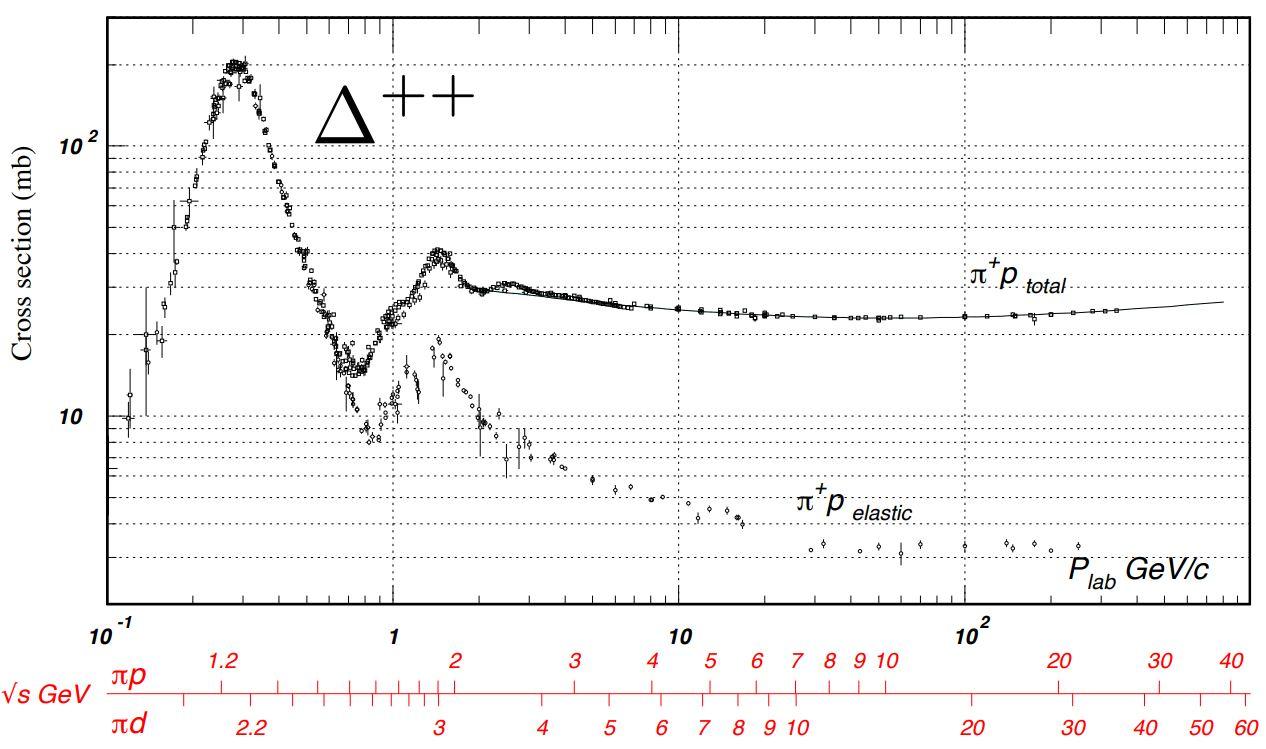
\includegraphics[width=0.8\textwidth]{Figures/FNSN31_8.JPG}
    \label{fig:Wu6}
    \caption{Measurement of the $\pi^+p$  interaction cross section}
\end{figure} 
\vspace{3mm}

\section{Discovery of the anti-proton (1955)}

The Bevatron (Synchrotron at the BeV, where BeV stands for Billion electron volt) was a particle accelerator — specifically, a weak-focusing proton synchrotron — at Lawrence Berkeley National Laboratory, U.S., which began operating in 1954. The antiproton was discovered there in 1955, resulting in the 1959 Nobel Prize in physics for Emilio Segrè and Owen Chamberlain. It accelerated protons into a fixed target, and was named for its ability to impart energies of billions of eV. 

\begin{figure}[!h]
    \centering
    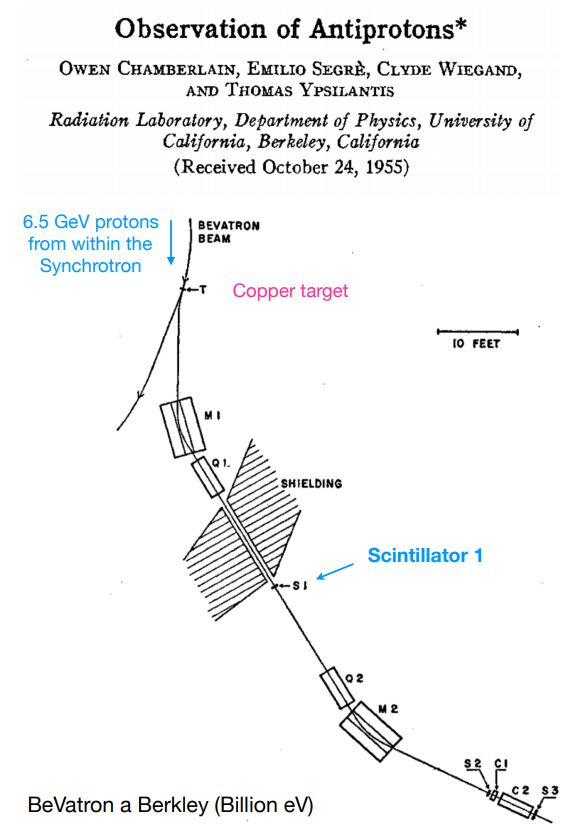
\includegraphics[width=0.5\textwidth]{Figures/FNSN31_9.JPG}
    \label{fig:antip0}
    \caption{Chamberlain, Segrè, Wiegland, Ypsilantis experiment on the observation of Antiprotons}
\end{figure} 

The Bevatron produces antiprotons with momentum $\sim 1.2 \ GeV$ and measures the momentum and the velocity with a system of Time-of-Flight (TOF) detectors. Figure \ref{fig:antip0} shows the experimental apparatus: protons are expected to have \SI{50}{ns} of TOF, while pions of \SI{40}{ns}, so this measured quantity can be used to discriminate the two kinds of particles (thus reducing background from pions).

Figure \ref{fig:antip1} shows on the left the measured mass of the antiproton, relative to the proton mass. On the right, a result from a contemporary experiment with emulsions by Amaldi et al. is shown: the photograph shows the evidence of the production of an anti-proton from cosmic rays.


\begin{figure}[!h]
    \centering
    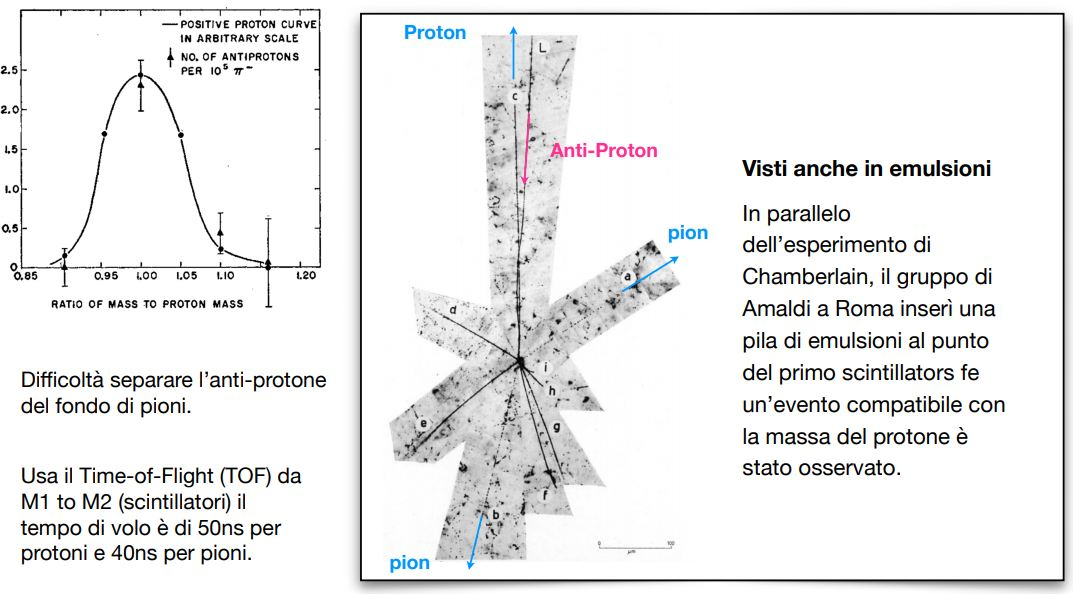
\includegraphics[width=0.6\textwidth]{Figures/FNSN31_10.JPG}
    \label{fig:antip1}
    \caption{BeVatron experiment}
\end{figure}

\section{Discovery of the $\Omega^-$}
More complex resonances were found with similar approaches. Fig. \ref{fig:omega-0} shows the experimental apparatus, based on a bubble chamber operated at the Brookhaven National Laboratory, used for the discovery of the $\Omega^-$ resonance. The resonance was produced with a kaon beam and can identified by its cascade decays, a photograph of which is shown in Fig. \ref{fig:omega-1} together with its interpretation in terms of identified particles. A detailed analysis of the decays showed that the strangeness of this particle was $S=-3$.

\begin{figure}[ht]
    \centering
    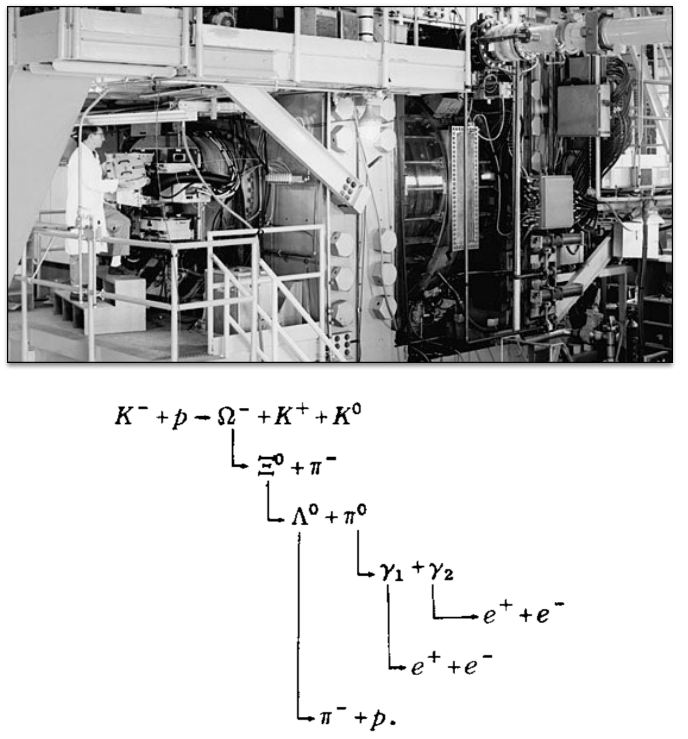
\includegraphics[width=0.6\textwidth]{Figures/FNSN31_11.JPG}
    \label{fig:omega-0}
    \caption{Illustration of different decays from the reaction $K^-+p$}
\end{figure}
 
\begin{figure}[!h]
    \centering
    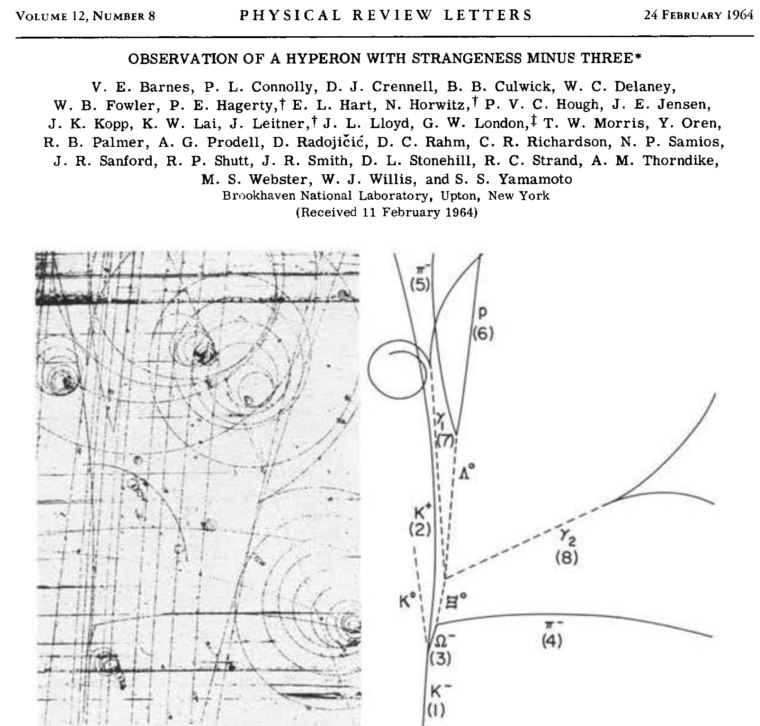
\includegraphics[width=0.6\textwidth]{Figures/FNSN31_12.JPG}
    \label{fig:omega-1}
    \caption{Illustration of the scientific article on observation of strangeness of $-3$.}
\end{figure}

\section{Discovery of the muon neutrino}

Pions collimated beam can be used to produce a neutrino beam,  since pions most often decay into muon neutrinos:

\[\pi^+ \rightarrow \mu^+\nu_{\mu}\]

Let's consider the frame of reference of the pion, as shown in figure \ref{fig:muon}.

\begin{figure}[!h]
    \centering
    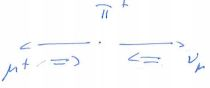
\includegraphics[width=0.4\textwidth]{Figures/FNSN31_13.JPG}
    \label{fig:muon}
    \caption{$\pi^+$ decay}
\end{figure}

The negative pion has spin zero; therefore the lepton and the antineutrino must be emitted with opposite spins (and opposite linear momenta) to preserve net zero spin (and conserve linear momentum). However, because the weak interaction is sensitive only to the left chirality component of fields, the neutrino has always left-handed. This implies that the muon must be emitted with spin in the direction of its linear momentum (i.e., also left-handed).

The polarization of fermions in the direction of motion is:

\[\left \langle \hat{p} \cdot \hat{s} \right \rangle = \frac{N_{n = 1}-N_{n = -1}}{N_{n = 1} + N_{n = -1}}\]

For a fermion (as $e^-$, $\nu_e$)
 \[\left \langle \hat{p_f} \cdot \hat{s_f} \right \rangle = -\beta \]
 
i.e. weak interaction is mostly producing left-handed fermions.
For anti-fermions, the previous formula becomes
 \[\left \langle \hat{p_{af}} \cdot \hat{s_{af}} \right \rangle = \beta \]
 
i.e. weak interaction is mostly producing right-handed anti-fermions.


Since the $\pi^+$ decay is weak and $\beta_{\nu} \sim 1$, the neutrino must be left-handed, and hence the anti-muon must be left-handed, too.
Therefore, the decay $\pi^+ \rightarrow e^+\nu_e$, having a bigger $\beta$ value (the positron) is less likely to happen, compared to the pion decaying into muons.

Once we are able to produce a neutrinos beam, along with muons, it shall be verified that it can have a reaction like

\[ \nu + p \rightarrow \mu^- + X \]

Figure \ref{fig:muoni} shows an example of such event: when a neutrino interacts with matter (the proton in the figure), a muon is produced along with other particles. This suggests the existence of a second type of neutrinos, the muon neutrino, as opposed to the electron neutrino (the one which, when interacting with matter, produces electrons). We now know that there are three families of leptons - electrons, muons, tauons, each associated with their corresponding neutrinos.


\begin{figure}[!h]
    \centering
    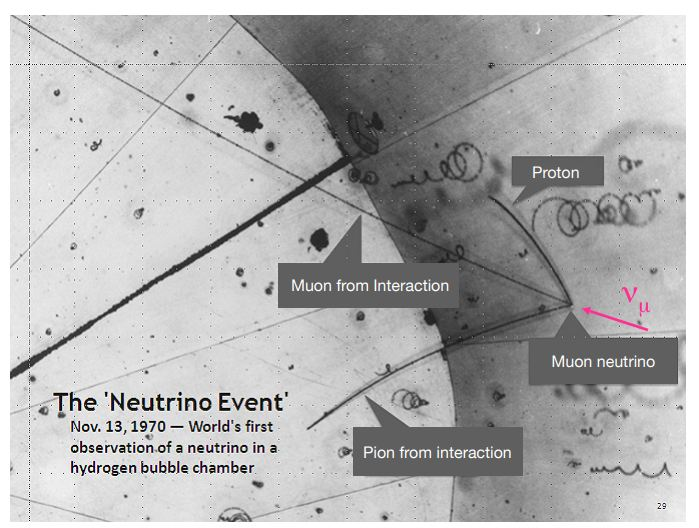
\includegraphics[width=0.6\textwidth]{Figures/FNSN31_14.JPG}
    \label{fig:muon1}
    \caption{Discovery of the neutrino}
\end{figure}
%\end{comment}